% vim:ts=4:sw=4
% Copyright (c) 2014 Casper Ti. Vector
% Public domain.

\chapter{附件}
% 中文测试文字。
\begin{table}[h]
\caption{实验结果}
\begin{tabularx}{17cm}{lllll}
\hline
场景名称   & 编辑时长(分)  & 覆盖面积(平方公里) &高程笔迹数(个)&纹理笔迹数(个)\\
\hline
梯田\\(图1)     & 25 & 4  & 14 & 547            \\
\hline
导弹发射基地\\(图2) & 35 & 16  & 122 & 1189     \\
\hline
虚拟战场\\(图3)   & 90 & 30    & 0  & 2521     \\
\hline
\end{tabularx}
\end{table}

\begin{table}[h]
\caption{编辑器测试环境及运行时参数}
\begin{tabularx}{17cm}{lllll}
\hline
名称&参数 \\
\hline
测试环境&CPU:Intel core i7-8700\\&RAM:16GB\\&GPU:NVIDIA GeForce GTX 1060            \\&操作系统:Windows10 64bit \\
\hline
窗口分辨率&   1680*813 \\
\hline
浏览帧率& 60-120帧/秒     \\
\hline
编辑帧率&25-65帧/秒    \\
\hline

\end{tabularx}
\end{table}

%------------------------
%\begin{table}[h]
%\caption{编辑器测试环境及结果}
%\begin{tabular}{@{}|l|l|l|@{}}
%\toprule
%\multicolumn{2}{|l|}{名称}     & 参数              \\ %\midrule
%\multirow{4}{*}{测试环境} & 操作系统 & Windows10 64bit %\\ \cmidrule(l){2-3}
%                      & CPU  &                 \\ \cmidrule(l){2-3}
%                      & GPU  &                 \\ \cmidrule(l){2-3}
%                      & RAM  &                 \\ \midrule
%\multicolumn{2}{|l|}{窗口分辨率}  & 1680*813        \\ %\midrule
%\multicolumn{2}{|l|}{帧率}     & 60hz            \\ \bottomrule
%\end{tabular}
%\end{table}
%--------------------------------------

\begin{figure}[h]
    \centering
    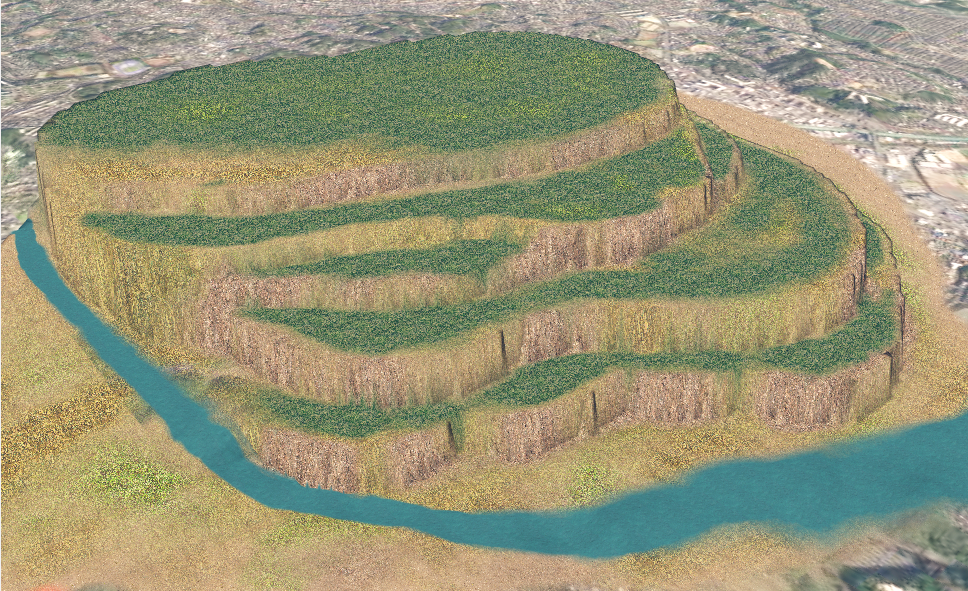
\includegraphics[height=7.5cm ,width=11.5cm]{figures/titian.PNG}
  \caption{平整笔刷构造出的梯田场景}
\end{figure}

\begin{figure}[h]
\centering
\subcaptionbox{}{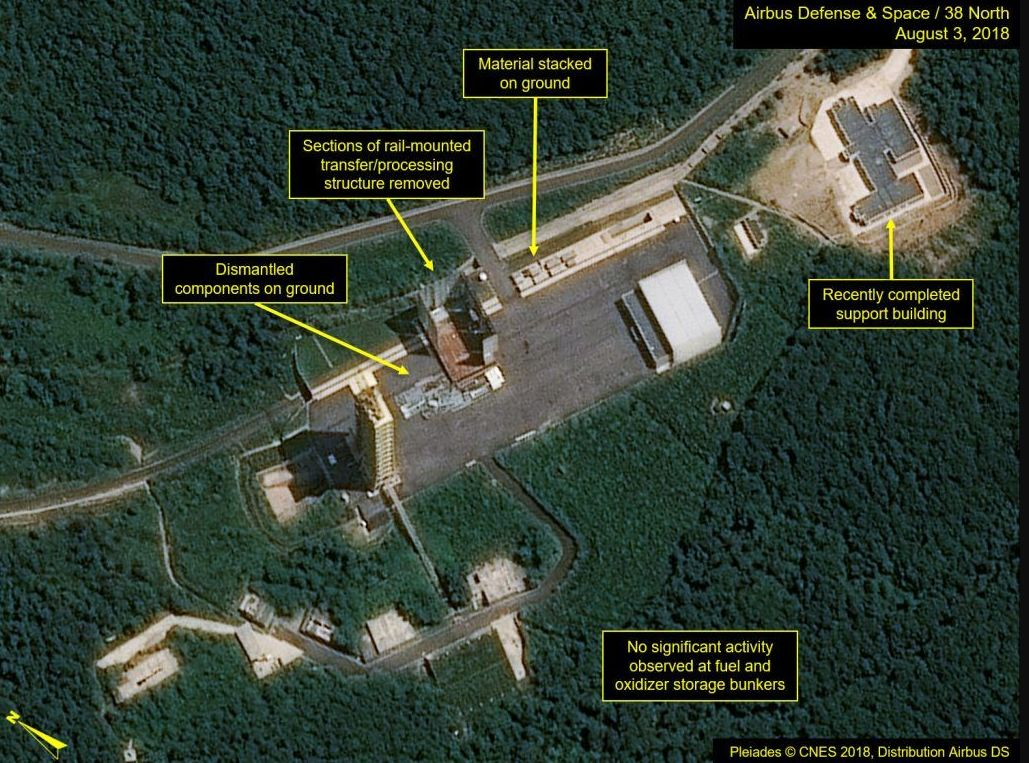
\includegraphics[height=5cm        ,width=6.8cm]{figures/q9-N-hnvukfe9576574.jpg}}
\subcaptionbox{}{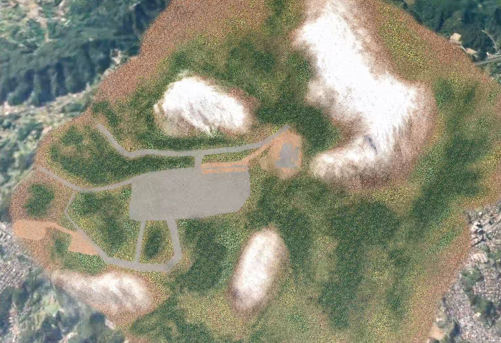
\includegraphics[height=5cm        ,width=7cm]{figures/result4.png}}
\subcaptionbox{}{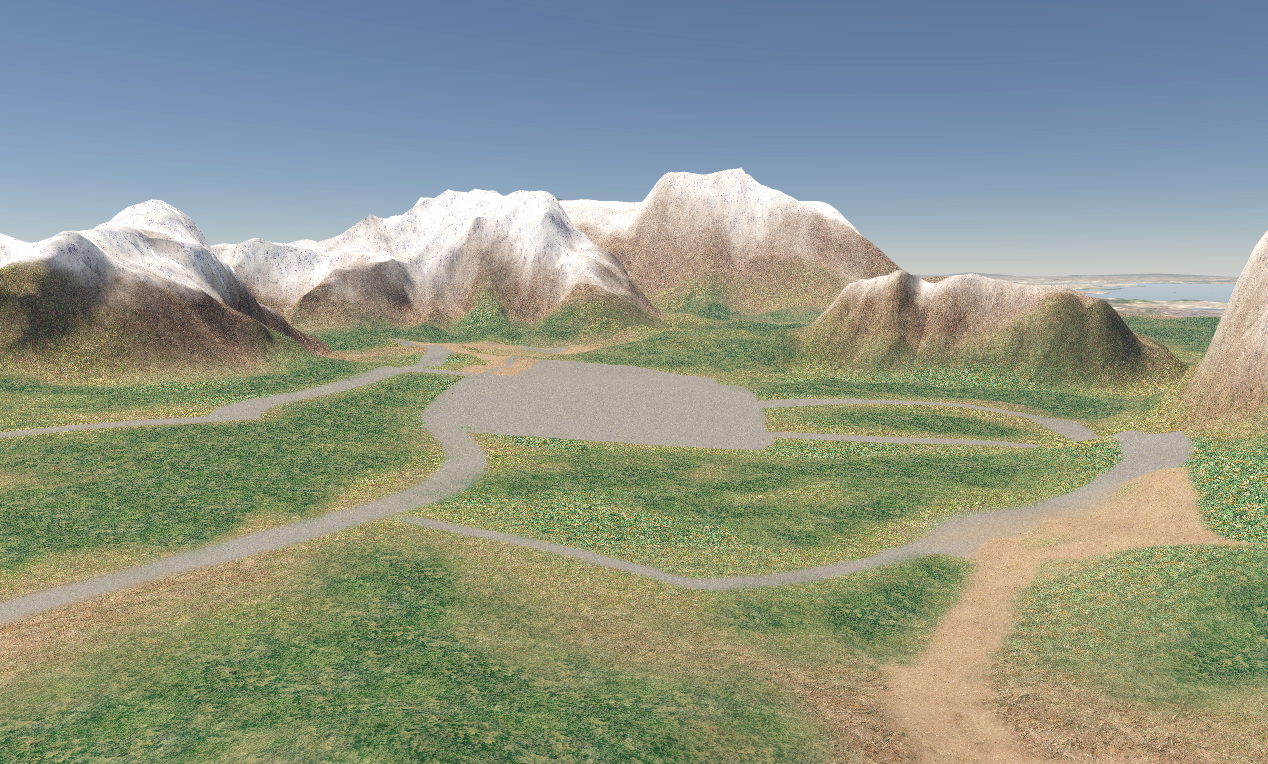
\includegraphics[height=5cm        ,width=7cm]{figures/result3.PNG}}
\subcaptionbox{}{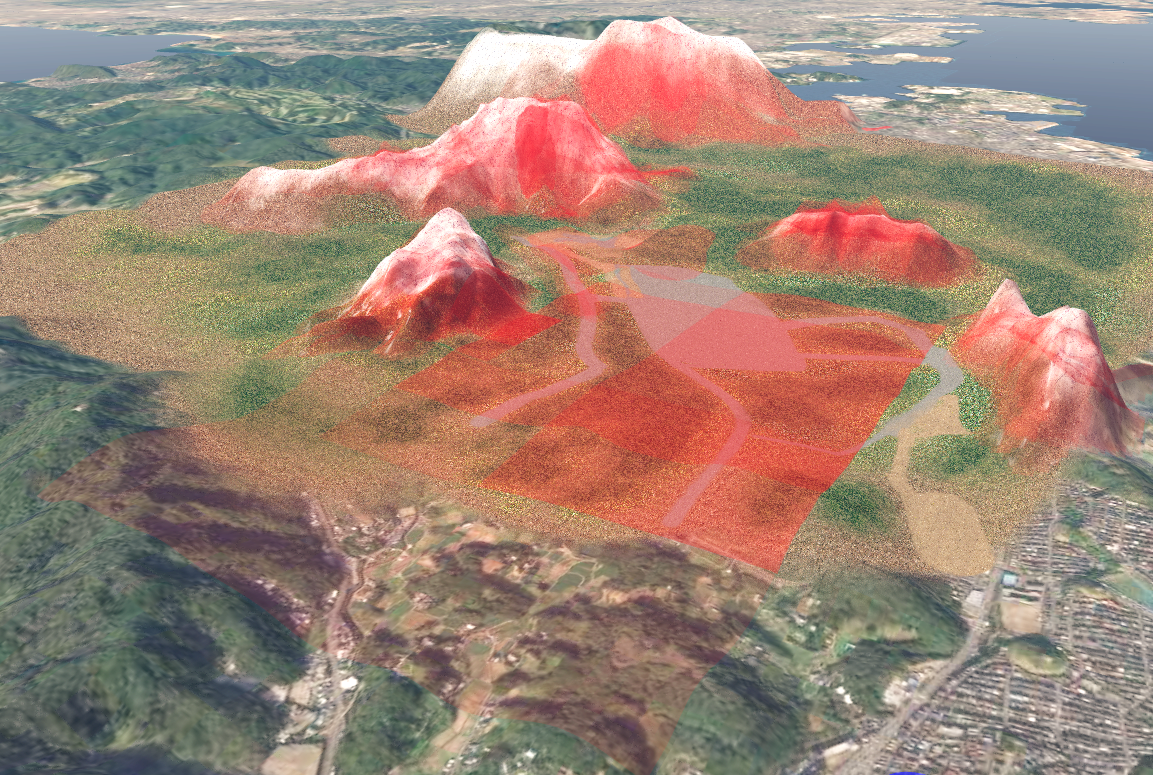
\includegraphics[height=5cm        ,width=7cm]{figures/editingArea.PNG}}

\caption{根据导弹发射基地卫星影像在Viwo中用地形编辑器构造的地形场景,(a).参考卫星影像(b).场景全景(c).山脉和道路细节(d).红色区域显示了场景的高程笔刷和选区编辑的历史}
\end{figure}

\begin{figure}[h]
    \centering
\subcaptionbox{}{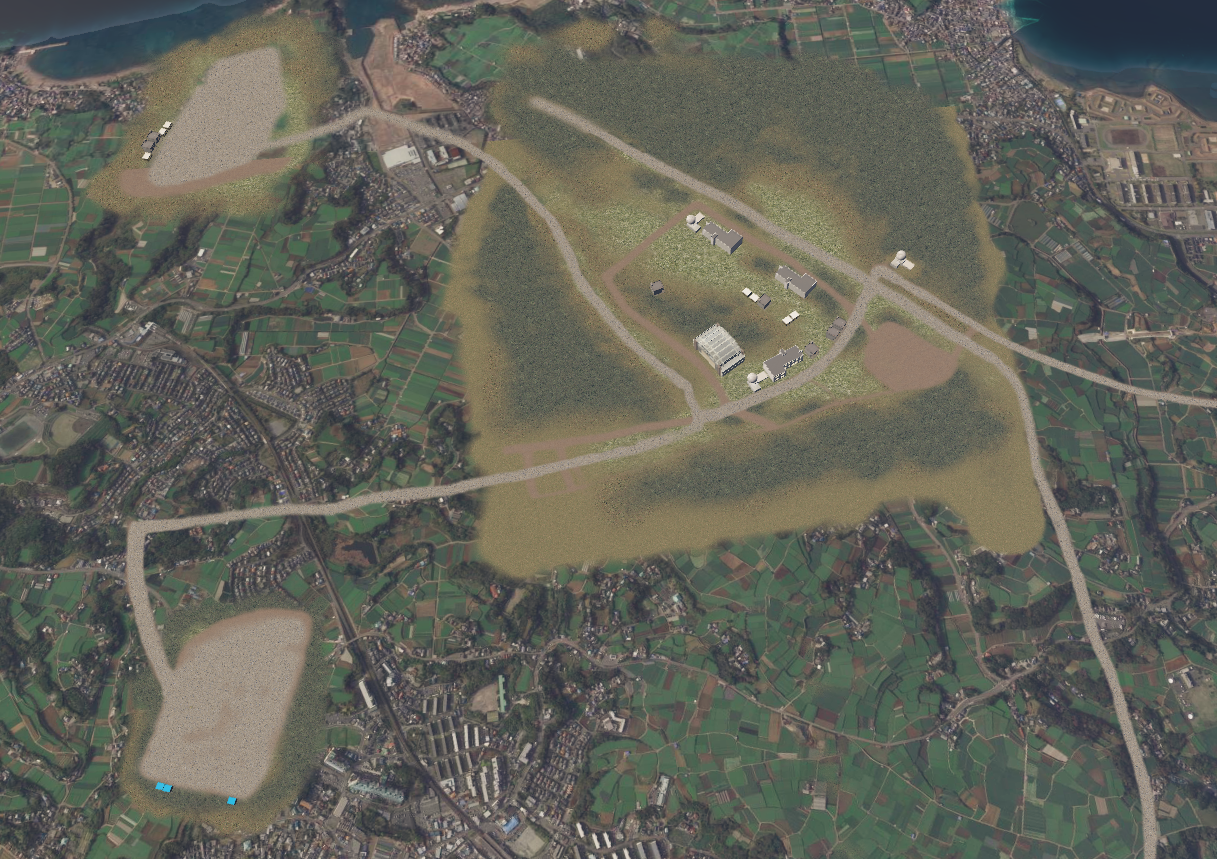
\includegraphics[height=5.4cm        ,width=7.6cm]{figures/base2.png}}
\subcaptionbox{}{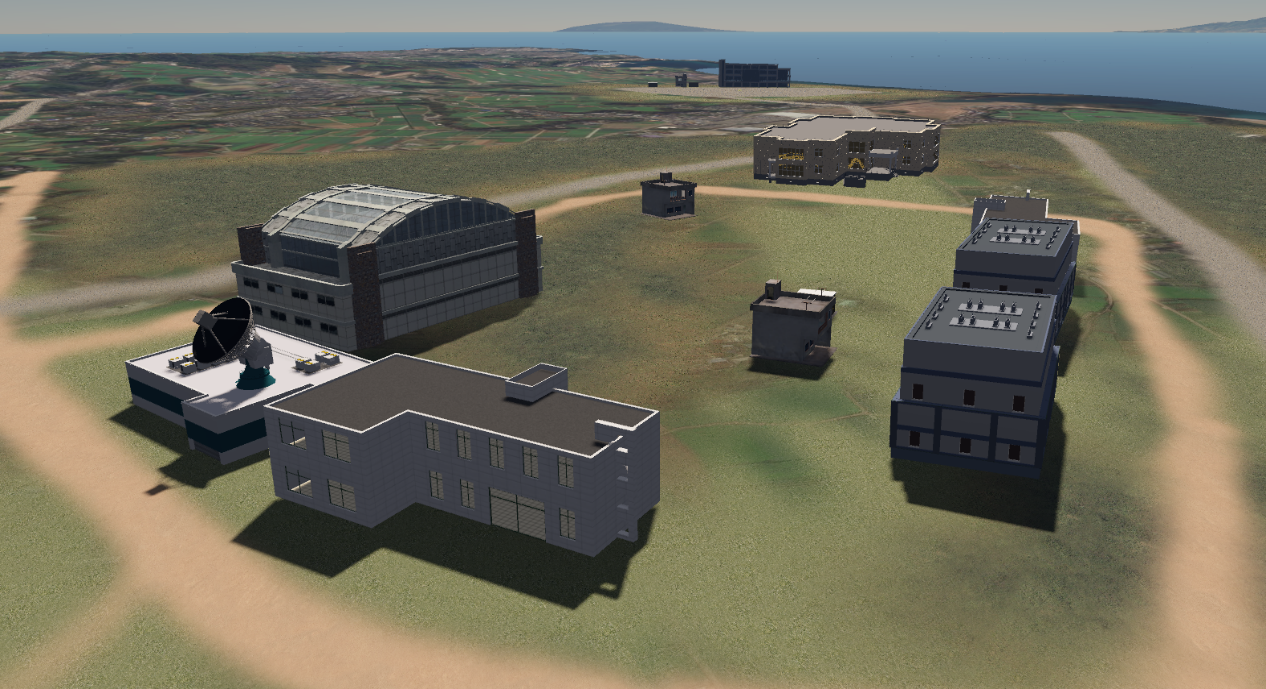
\includegraphics[height=5.4cm        ,width=7.6cm]{figures/base.png}}\\
\subcaptionbox{}{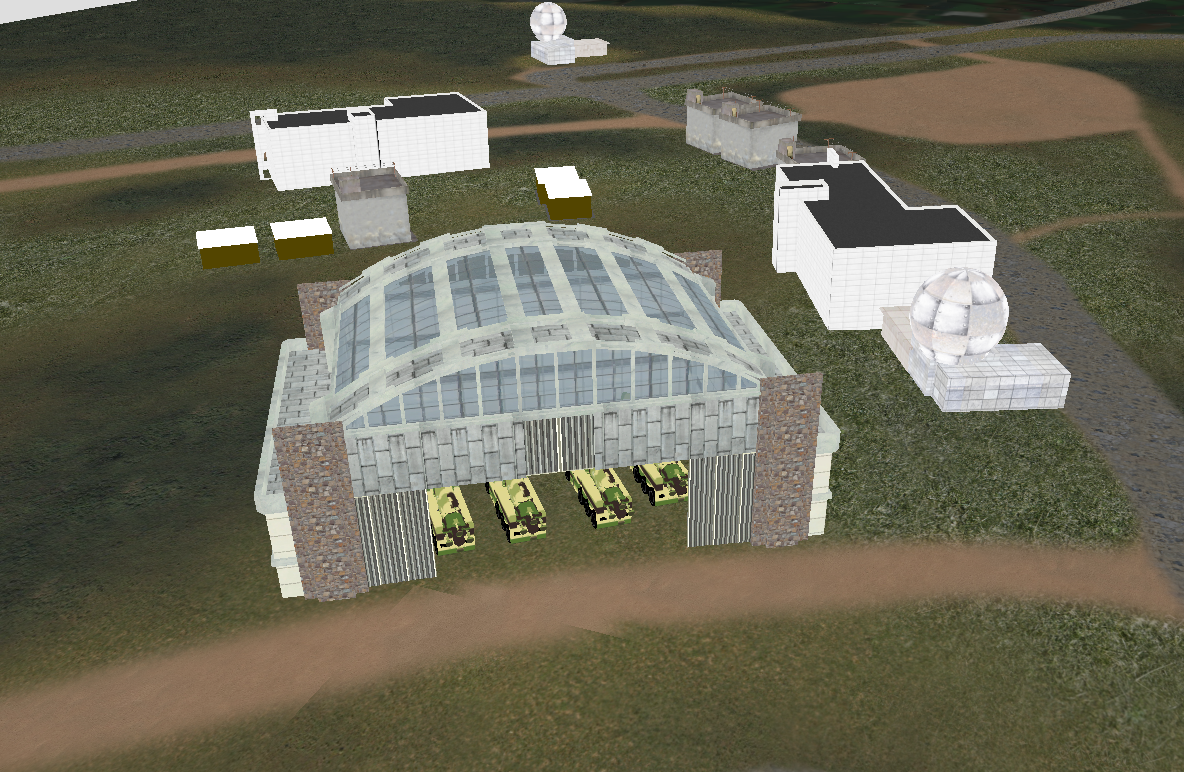
\includegraphics[height=5.5cm        ,width=7.8cm]{figures/base5.png}}
\subcaptionbox{}{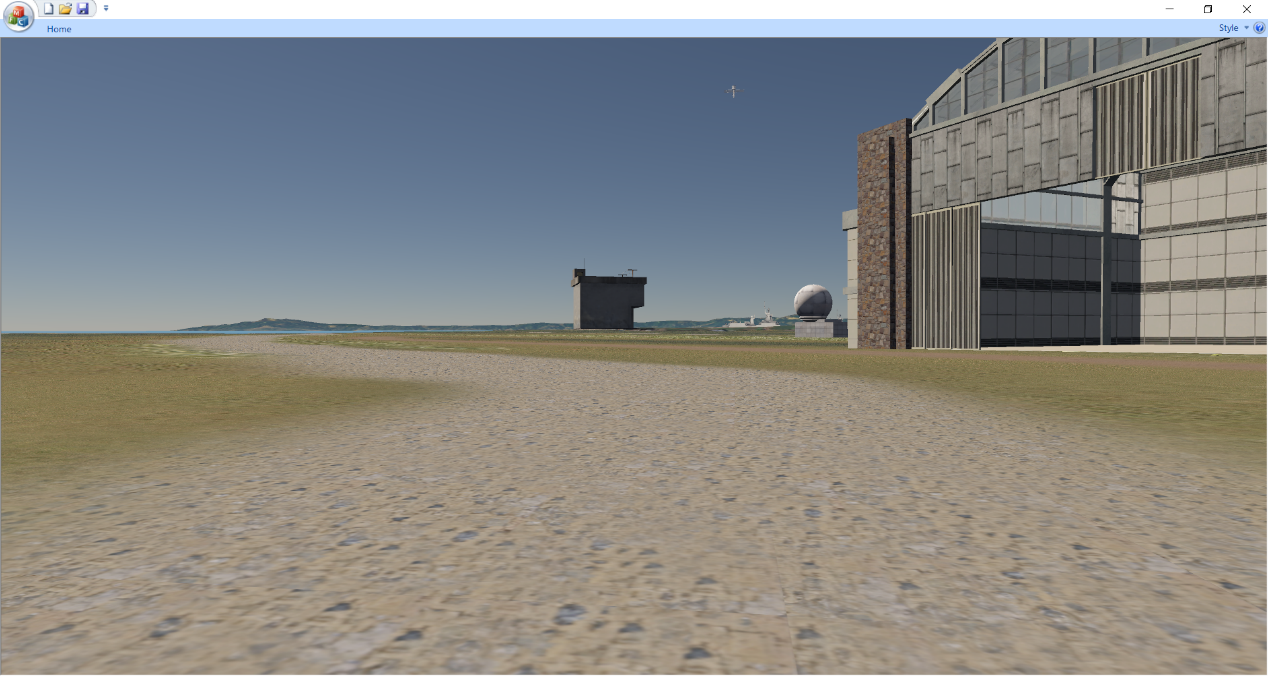
\includegraphics[height=5.5cm        ,width=7.9cm]{figures/base3.png}}
  \caption{地形编辑器在与中国空间技术研究院合作的战场模拟项目中用于构建模拟战场环境(a).模拟战场全景(b).模拟战场近景(c).导弹车隐蔽在车库中的场景(d).贴近地表漫游}
\end{figure}
%& 高程工程文件大小(MB)& 纹理工程文件大小(MB)


